\section{Ranking TechEmpower}

TechEmpower to projekt Benchmarków Frameworków Webowych który jest otwartym źródłem \cite{techempower}.
Projekt ten mierzy wydajność wielu języków i frameworków aplikacji, co pozwala na ocenę wpływu wyboru technologii na wyniki wydajności.
Benchmarki te są szeroko oglądane przez programistów aplikacji internetowych i cieszą się dużym zainteresowaniem w branży.
Celem TechEmpower jest dostarczenie obiektywnych danych na temat wydajności różnych narzędzi i technologii, aby pomóc programistom w dokonywaniu świadomych wyborów technologicznych podczas budowy aplikacji internetowych.

Wybrane w tej pracy frameworki znajdują się w zestawieniu.
Najwyżej w rankingu uplasował się .Net umieszczony na 155 miejscu z wynikiem wydajności 42,23\%.
Kolejnym frameworkiem okazał się NestJS znajdując się na 419 miejscu z wydajnością 10,8\%.
Najniżej w rankingu znalazł się Django zajmując 472 miejsce z wydajnością na poziomie 4,3\%. 

Od 2013 roku, kiedy zostało opublikowane pierwsze zestawienie, badane są regularnie narzędzia.
Początkowo badany był czas serializacji danych i zapytania do bazy danych.
Z czasem porównanie zaczęło być rozszerzane o kolejne testy.
Badanie odbywa się regularnie tworząc wiele rund dzięki czemu jego wyniki są regularnie aktualizowane.
Dzięki regularnemu publikowaniu wyników, gotowe są narzędzia do wizualizacji wyników badania.
W czasie rzeczywistym można śledzić postępy badania wraz z informacją ile testów przeszło oraz ile nie udało się wykonać.
Przykładowy fragment z podglądu testów został zaprezentowany na rysunku \ref{rys:techempowerdashhboard}.

\begin{figure}[!hb]
	\centering 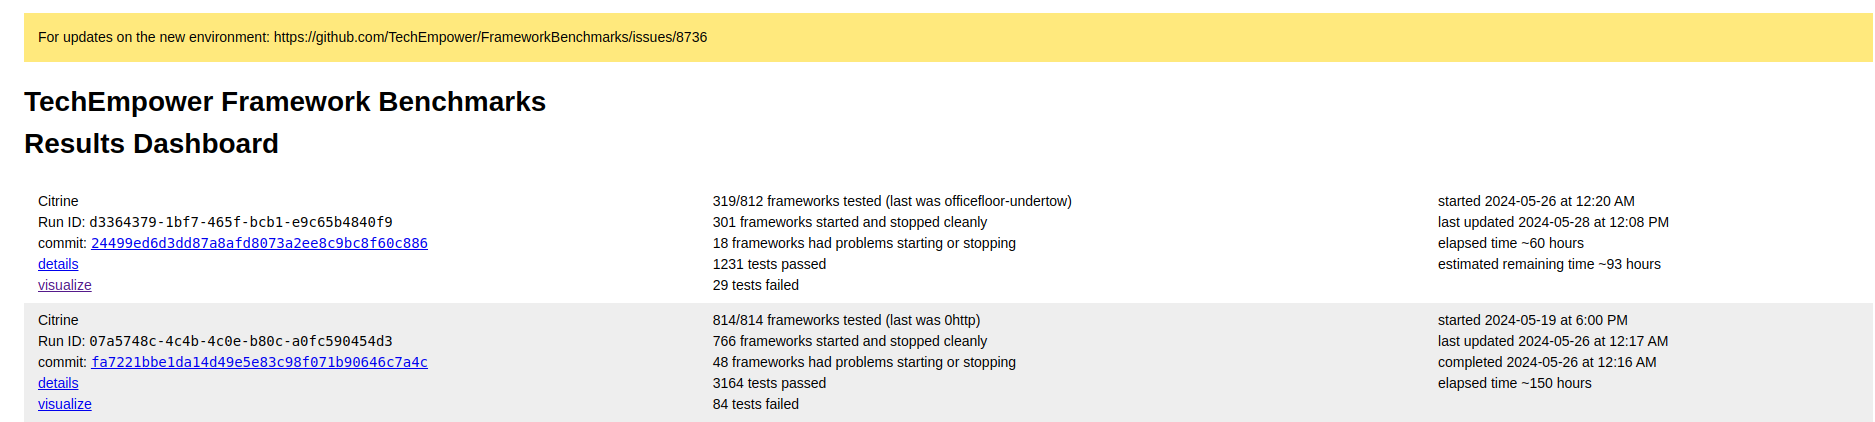
\includegraphics[width=1\linewidth]{rysunki/techempower_result_daschboard.png}
	\caption{Fragment podglądu testów TechEmpower - źródło: \cite{techempower}.}
	\label{rys:techempowerdashhboard}
\end{figure}

Widoczny jest nacisk położony na przejrzystość wyników.